%!TEX program = xelatex
\immediate\write18{makeindex -s nomencl.ist -o "\jobname.nls" "\jobname.nlo"}
\documentclass{Classes/UITBA}

%====================================  Common information

\def\organization{Đại học Quốc gia TP. Hồ Chí Minh}
\def\university{Trường Đại học Công nghệ thông tin}
\def\department{Khoa Khoa học máy tính}
\newarray\title
\readarray{title}{Tìm hiểu nhận diện khuôn mặt bằng phương pháp Deep Learning&A Study on Face Recognition using Deep Learning}
\newarray\student
 \newcommand{\numberstudent}{2} % Number of students
\readarray{student}{13521064&Nguyễn Thụy Vy&MSSV2&TenSinhVien2}
\newarray\instructor
 \newcommand{\numberinstructor}{2} % Number of instructors
\readarray{instructor}{PGS. TS. Dương Anh Đức&Assoc. Prof. Duong Anh Duc&GVHD2&SecondInstructor}
\newarray\board
\readarray{board}{Chủ tịch&PGS.TS. Đỗ Phúc&Thư ký&ThS. Trịnh Quốc Sơn&Ủy viên&TS. Nguyễn Hoàng Tú Anh}
\def\date{25/8/2014 }
\def\place{TP. Hồ Chí Minh}
\def\year{2017}
\dataheight=2


%==================================== Bibliography

\usepackage[backend=biber,style=numeric-comp,sorting=sample]{biblatex}
\DeclareSortingScheme{sample}{
	\sort{
	\field{title}
	}
	\sort{
	\field{author}
	}
	\sort{
	\field{year}
	}
	\sort{\citeorder}
}
\addbibresource{Reference/Reference.bib}

%==================================== Nomenclature

\usepackage{nomencl}
\makenomenclature

%==================================== Math stuff

\usepackage{mathastext}

%==================================== Table of contents

\setcounter{secnumdepth}{5}
\setcounter{tocdepth}{5}

\begin{document}
\selectlanguage{vietnamese}

%\begin{otherlanguage}{vietnamese} %Uncomment this line and its corresponding ending line if \selectlanguage{english}

\pagestyle{empty}
\newgeometry{left=3cm,right=3cm,top=3cm,bottom=3cm}
\begin{titlepage}\uctimes

\thisfancyput(3.2in,-4.75in){\setlength{\unitlength}{1in}\fancyoval(7,10.1)}

\large\organization

\Large\university

\Large\department

\vspace{1cm}

\normalsize\student(2) - \student(1)

\vspace{1cm}

\Large Khóa luận tốt nghiệp

\Huge\title(1)

\vspace{0.5cm}

\normalsize(\title(2))

\vspace{2cm}

Cử nhân ngành Khoa học máy tính

\vspace{2cm}

Giảng viên hướng dẫn

\instructor(1)

\vfill

TP. Hồ Chí Minh, 2017

\end{titlepage}
\clearpage
\restoregeometry

\nheading{Danh sách Hội đồng bảo vệ Khóa luận}

Hội đồng chấm khóa luận tốt nghiệp, thành lập theo Quyết định số ………… ngày \date của Hiệu trưởng \university.

\begin{enumerate}
	\item \board(1, 2) - \board(1, 1)
	\item \board(2, 2) - \board(2, 1)
	\item \board(3, 2) - \board(3, 1)
\end{enumerate}

\nheading{Acknowledgement}

Here I would like to show my appreciation to my instructor – \instructor(2) and mister Ph.D. Thanh Duc Ngo and to all members of Multimedia Communications Laboratory (MMLaB) of University of Information Technology, especially mister M.S. Nguyen Vinh Tiep, mister M.S. Do Van Tien, miss M.S. Nguyen Thi Bao Ngoc and all students of the class KHTN2013 for making this work possible. 
\nheading{Nhận xét}
\begin{center}\textbf{(Của giảng viên hướng dẫn)}\end{center}

\fillwithdottedlines

\nheading{Nhận xét}
\begin{center}\textbf{(Của giảng viên phản biện)}\end{center}

\fillwithdottedlines

%\end{otherlanguage}

\pagestyle{empty}
\tableofcontents
\listoffigures
\listoftables
\renewcommand{\nomname}{\IfLanguageName{vietnamese}{Danh sách các từ viết tắt}{Abbreviations}}
\printnomenclature[2cm]
 
\clearpage
\pagestyle{plain}
\setcounter{page}{1}

\heading{Abstract}

Sed ut perspiciatis, unde omnis iste natus error sit voluptatem accusantium doloremque laudantium, totam rem aperiam eaque ipsa, quae ab illo inventore veritatis et quasi architecto beatae vitae dicta sunt, explicabo. Nemo enim ipsam voluptatem, quia voluptas sit, aspernatur aut odit aut fugit, sed quia consequuntur magni dolores eos, qui ratione voluptatem sequi nesciunt, neque porro quisquam est, qui dolorem ipsum, quia dolor sit amet consectetur adipisci[ng] velit, sed quia non numquam [do] eius modi tempora inci[di]dunt, ut labore et dolore magnam
\chapter{Mở đầu}

\section{Tên khóa luận}

vel illum, qui dolorem eum fugiat, quo voluptas nulla pariatur?

\section{Tổng quan về khóa luận}

\subsection{Đặt vấn đề}

Sed ut perspiciatis, unde omnis iste natus error sit voluptatem accusantium doloremque laudantium, totam rem aperiam eaque ipsa, quae ab illo inventore veritatis et quasi architecto beatae vitae dicta sunt, explicabo. Nemo enim ipsam voluptatem, quia voluptas sit, aspernatur aut odit aut fugit, sed quia consequuntur magni dolores eos, qui ratione voluptatem sequi nesciunt, neque porro quisquam est, qui dolorem ipsum, quia dolor sit amet consectetur adipisci[ng] velit, sed quia non numquam [do] eius modi tempora inci[di]dunt, ut labore et dolore magnam {\textbf aliquam quaerat voluptatem}. Ut enim ad minima veniam, quis nostrum exercitationem ullam corporis suscipit laboriosam, nisi ut aliquid ex ea commodi consequatur? Quis autem vel eum iure reprehenderit, qui in ea voluptate velit esse, quam nihil molestiae consequatur, vel illum, qui dolorem eum fugiat, quo voluptas nulla pariatur? (\autoref{fig:11}, Hình \ref{fig:12})

$\Rightarrow$ vel illum, qui dolorem eum fugiat, quo voluptas nulla pariatur?

\begin{figure}
  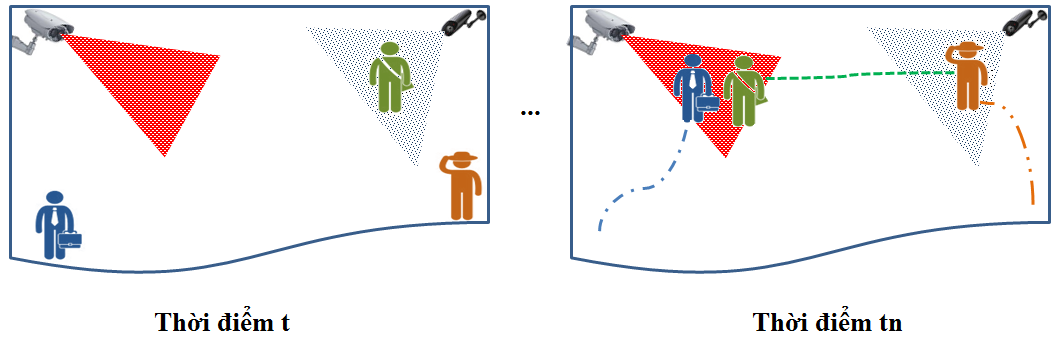
\includegraphics[width=\linewidth]{Chapter1/Figure/1.png}
  \caption{vel illum, qui dolorem eum fugiat, quo voluptas nulla pariatur?}
  \label{fig:11}
\end{figure}

\begin{figure}
  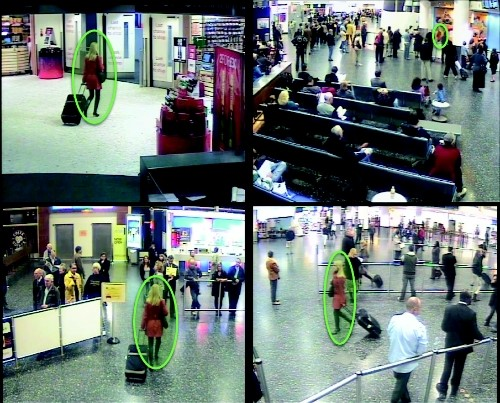
\includegraphics[width=\linewidth]{Chapter1/Figure/2.jpg}
  \caption{vel illum, qui dolorem eum fugiat, quo voluptas nulla pariatur?}
  \label{fig:12}
\end{figure}

\begin{itemize}
	\item vel illum, qui dolorem eum fugiat, quo voluptas nulla pariatur?
	\item vel illum, qui dolorem eum fugiat, quo voluptas nulla pariatur?
	\begin{itemize}
		\item vel illum, qui dolorem eum fugiat, quo voluptas nulla pariatur?
	\end{itemize}
\end{itemize}


\subsection{Nội dung khóa luận}

Sed ut perspiciatis, unde omnis iste natus error sit voluptatem accusantium doloremque laudantium, totam rem aperiam eaque ipsa, quae ab illo inventore veritatis et quasi architecto beatae vitae dicta sunt, explicabo. Nemo enim ipsam voluptatem, quia voluptas sit, aspernatur aut odit aut fugit, sed quia consequuntur magni dolores eos, qui ratione voluptatem sequi nesciunt, neque porro quisquam est, qui dolorem ipsum, quia dolor sit amet consectetur adipisci[ng] velit, sed quia non numquam [do] eius modi tempora inci[di]dunt, ut labore et dolore magnam \autoref{chap:attrel}. \cite{knuthwebsite}\cite{latexcompanion} \cite{knuthwebsite,latexcompanion}

Convolutional Neural Network (CNN) is a kind of neural network involves convolution. \nomenclature{CNN}{Convolutional Neural Network}

\begin{table}
\centering
\begin{tabular}{ |p{3cm}|p{3cm}|p{3cm}|  }
\hline
\multicolumn{3}{|c|}{Country List} \\
\hline
Country Name     or Area Name& ISO ALPHA 2 Code &ISO ALPHA 3 \\
\hline
Afghanistan & AF &AFG \\
Aland Islands & AX   & ALA \\
Albania &AL & ALB \\
Algeria    &DZ & DZA \\
American Samoa & AS & ASM \\
Andorra & AD & AND   \\
Angola & AO & AGO \\
\hline
\end{tabular}
\caption{Ahihi đồ ngốc}
  \label{tab:11}
  \end{table}
\chapter{Tổng quan}

\section{Giới thiệu chung về phương pháp đề xuất}

Sed ut perspiciatis, unde omnis iste natus error sit voluptatem accusantium doloremque laudantium, totam rem aperiam eaque ipsa, quae ab illo inventore veritatis et quasi architecto beatae vitae dicta sunt, explicabo. Nemo enim ipsam voluptatem, quia voluptas sit, aspernatur aut odit aut fugit, 
\chapter{Phương pháp đề xuất}
\label{chap:attrel}

\section{Giới thiệu chung về phương pháp đề xuất}

Sed ut perspiciatis, unde omnis iste natus error sit voluptatem accusantium doloremque laudantium, totam rem aperiam eaque ipsa, quae ab illo inventore veritatis et quasi architecto beatae vitae dicta sunt, explicabo. Nemo enim ipsam voluptatem, quia voluptas sit, aspernatur aut odit aut fugit, 

\printbibliography

\end{document}
